%% toc: P2 12 12.1,12.2,12.3,12.4
\section{Derivation trees and the intuitionistic boundary of classical natural deduction}
\label{sec:p02-w02b-p02-008-trees-and-boundary}

The classical calculus \(\mathsf{ND}_{\mathsf{CPL}}\) of
\cref{sec:prop-deduction-01} is defined by finite rooted trees whose leaves
are assumption occurrences and whose discharges are recorded by labels.  The
two worked examples of that section are printed as numbered lines.  This
section does two things.  First, it displays both examples as the trees the
definition actually speaks about, with every discharge label shown, and
states exactly how each numbered line corresponds to tree nodes.  Second, it
proves the boundary claim made in the Excluded-middle example: the calculus
obtained by deleting \(\mathsf{RAA}\), with primitive \(\neg\) and the rules
\(\neg I\), \(\neg E\) and \(\bottom E\) kept, derives \(P\lor\neg P\) from no
open assumptions for no propositional variable \(P\).  The proof is a
soundness theorem for that calculus over the Kripke structures of
\cref{sec:intuitionistic-logic-01}, extended by a forcing clause for
primitive negation, followed by the two-world countermodel.

\emph{Inputs.}  Formulas of \(\mathsf{Fm}_{\mathsf{CPL}}\)
(\cref{sec:prop-syntax-semantics-01}), with primitive
\(\bottom,\neg,\land,\lor,\to\); natural-deduction derivations in the sense
of \cref{sec:prop-deduction-01}; and Kripke structures
\(\mathcal M=(W,\leq,V)\) as in \cref{sec:intuitionistic-logic-01}.
\emph{Conclusions.}  Tree displays of the two examples; Kripke soundness of
the calculus without \(\mathsf{RAA}\)
(\cref{thm:p02-w02b-p02-008-kripke-soundness}); and nonderivability of
\(P\lor\neg P\) and of \(\neg\neg P\to P\) in that calculus
(\cref{thm:p02-w02b-p02-008-nonderivability}).

\subsection{The worked derivations as trees}
\label{sec:p02-w02b-p02-008-trees}

\begin{hbconvention}{def:p02-w02b-p02-008-tree-display}{Reading a displayed derivation tree}
In \cref{fig:p02-w02b-p02-008-commutativity-tree,fig:p02-w02b-p02-008-excluded-middle-tree}
every formula is one node.  A horizontal line has the premises of one rule
application above it and its conclusion below it; the name at the right of
the line is the rule, followed, for a discharging rule, by the label it
carries.  A formula written \([\varphi]^i\) is an assumption occurrence
marked \(i\); an unbracketed formula with no line above it would be an
unmarked assumption occurrence, and none occurs in these two trees.  Rule
names are those of the calculus sheet
\texttt{sheet:\allowbreak nd-cpl}.  An assumption occurrence is open iff no
application on its path to the root discharges it
(\cref{sec:prop-deduction-01}).  For a derivation \(D\),
\(\operatorname{oa}(D)\) is the finite set of formulas that have at least one
open assumption occurrence in \(D\), as in \cref{def:p02-fbc-language}.
\end{hbconvention}

\begin{figure}[htbp]
\centering
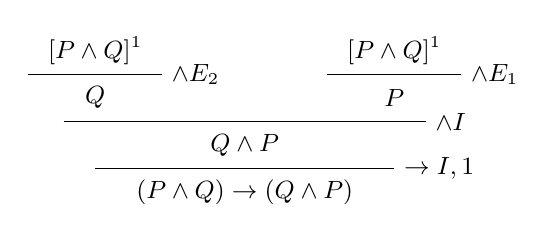
\begin{tikzpicture}[font=\small]
  \node at (-1.9,2.80) {\([P\land Q]^1\)};
  \node at ( 1.9,2.80) {\([P\land Q]^1\)};
  \draw (-2.75,2.50) -- (-1.05,2.50);
  \node[right] at (-1.05,2.50)
    {\(\land E_2\)};
  \draw (1.05,2.50) -- (2.75,2.50);
  \node[right] at (2.75,2.50)
    {\(\land E_1\)};
  \node at (-1.9,2.20) {\(Q\)};
  \node at ( 1.9,2.20) {\(P\)};
  \draw (-2.3,1.90) -- (2.3,1.90);
  \node[right] at (2.3,1.90)
    {\(\land I\)};
  \node at (0,1.60) {\(Q\land P\)};
  \draw (-1.9,1.30) -- (1.9,1.30);
  \node[right] at (1.9,1.30)
    {\(\to I,1\)};
  \node at (0,1.00) {\((P\land Q)\to(Q\land P)\)};
\end{tikzpicture}
\caption{The derivation of \((P\land Q)\to(Q\land P)\) in
\(\mathsf{ND}_{\mathsf{CPL}}\) as a tree.  The two top nodes are distinct
assumption occurrences of \(P\land Q\), both marked \(1\); the final
\(\to I\) carries label \(1\) and discharges both, so the tree has no open
assumption.}
\label{fig:p02-w02b-p02-008-commutativity-tree}
\end{figure}

\begin{hbexample}{def:p02-w02b-p02-008-commutativity-map}{Commutativity of conjunction, line by line}
The Commutativity-of-conjunction example of \cref{sec:prop-deduction-01}
lists five lines.  They correspond to the nodes of
\cref{fig:p02-w02b-p02-008-commutativity-tree} as follows.
\begin{enumerate}
  \item Line 1, \([P\land Q]^1\), is cited twice, by lines 2 and 3.  A tree
        node has exactly one parent, so line 1 corresponds to two leaf
        occurrences, one above each elimination; both carry the label \(1\).
        This is the reading fixed by the definition of a derivation: there
        is no repetition step, and a formula cited twice is not one node
        with two parents.
  \item Line 2, \(Q\) by \(\land E_2\) from line 1, is the left node \(Q\)
        with the left leaf as its only premise.
  \item Line 3, \(P\) by \(\land E_1\) from line 1, is the right node \(P\)
        with the right leaf as its only premise.
  \item Line 4, \(Q\land P\) by \(\land I\) from lines 2 and 3, has premises
        in the order displayed by \(\land I\): first \(Q\), then \(P\).
  \item Line 5, \(\to I\) on lines 1--4, is the root application.  It
        carries label \(1\) and discharges exactly the open occurrences of
        \(P\land Q\) marked \(1\) above its premise, namely both leaves.
        Each carried label discharges at least one occurrence, as the
        definition requires.
\end{enumerate}
Since both leaves are discharged, \(\operatorname{oa}(D)=\varnothing\) for
this tree \(D\), which is the statement
\(\varnothing\derives_{\mathsf{ND}_{\mathsf{CPL}}}(P\land Q)\to(Q\land P)\).
No rule other than \(\land E_1,\land E_2,\land I,\to I\) occurs, so the same
tree is also a derivation of the calculus without \(\mathsf{RAA}\) defined
in \cref{def:p02-w02b-p02-008-nd-minus-raa}.
\end{hbexample}

\begin{figure}[htbp]
\centering
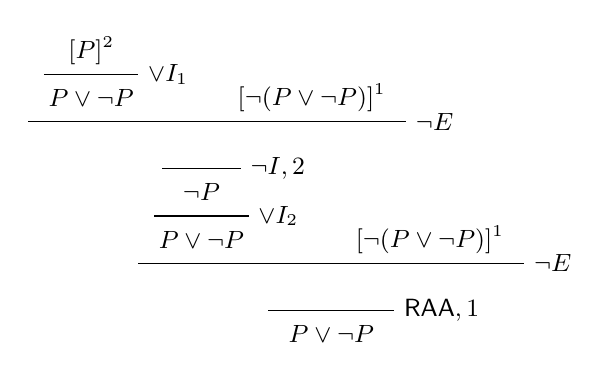
\begin{tikzpicture}[font=\small]
  \node at (-2.4,4.20) {\([P]^2\)};
  \draw (-3.0,3.90) -- (-1.8,3.90);
  \node[right] at (-1.8,3.90)
    {\(\lor I_1\)};
  \node at (-2.4,3.60) {\(P\lor\neg P\)};
  \node at ( 0.4,3.60) {\([\neg(P\lor\neg P)]^1\)};
  \draw (-3.2,3.30) -- (1.6,3.30);
  \node[right] at (1.6,3.30)
    {\(\neg E\)};
  \node at (-1.0,3.00) {\(\bottom\)};
  \draw (-1.5,2.70) -- (-0.5,2.70);
  \node[right] at (-0.5,2.70)
    {\(\neg I,2\)};
  \node at (-1.0,2.40) {\(\neg P\)};
  \draw (-1.6,2.10) -- (-0.4,2.10);
  \node[right] at (-0.4,2.10)
    {\(\lor I_2\)};
  \node at (-1.0,1.80) {\(P\lor\neg P\)};
  \node at ( 1.9,1.80) {\([\neg(P\lor\neg P)]^1\)};
  \draw (-1.8,1.50) -- (3.1,1.50);
  \node[right] at (3.1,1.50)
    {\(\neg E\)};
  \node at (0.65,1.20) {\(\bottom\)};
  \draw (-0.15,0.90) -- (1.45,0.90);
  \node[right] at (1.45,0.90)
    {\(\mathsf{RAA},1\)};
  \node at (0.65,0.60) {\(P\lor\neg P\)};
\end{tikzpicture}
\caption{The classical derivation of \(P\lor\neg P\) as a tree.  The two
occurrences of \(\neg(P\lor\neg P)\) are both marked \(1\) and are
discharged by the final \(\mathsf{RAA}\); the occurrence of \(P\) marked
\(2\) is discharged by \(\neg I\).  The final inference is the only
application of \(\mathsf{RAA}\).}
\label{fig:p02-w02b-p02-008-excluded-middle-tree}
\end{figure}

\begin{hbexample}{def:p02-w02b-p02-008-excluded-middle-map}{Excluded middle, line by line, and the role of the last step}
The Excluded-middle example of \cref{sec:prop-deduction-01} lists eight
lines.  Line 1, \([\neg(P\lor\neg P)]^1\), is cited by lines 4 and 7, so it
corresponds to the two leaves marked \(1\) in
\cref{fig:p02-w02b-p02-008-excluded-middle-tree}.  Line 2, \([P]^2\), is the
single leaf marked \(2\).  Lines 3, 5 and 6 are the nodes \(P\lor\neg P\)
(by \(\lor I_1\)), \(\neg P\) (by \(\neg I\) with label \(2\)) and
\(P\lor\neg P\) (by \(\lor I_2\)).  Lines 4 and 7 are the two applications of
\(\neg E\); the rule takes \(\varphi\) as its first premise and
\(\neg\varphi\) as its second, so in both the formula \(P\lor\neg P\) stands
left of \(\neg(P\lor\neg P)\).  Line 8 is the root, an application of
\(\mathsf{RAA}\) with label \(1\) discharging both leaves marked \(1\).

The application of \(\neg I\) with label \(2\) sits on the path of the left
leaf marked \(1\) but carries a different label, so it does not discharge
that leaf; only the root does.  Replacing the root inference
\(\mathsf{RAA},1\) by \(\neg I,1\), whose premise has the same shape
(\(\bottom\) above, open occurrences of \(\neg(P\lor\neg P)\) marked \(1\)),
gives a tree with conclusion \(\neg\neg(P\lor\neg P)\) and no open
assumption, in which \(\mathsf{RAA}\) does not occur.  So the calculus
without \(\mathsf{RAA}\) derives \(\neg\neg(P\lor\neg P)\) from no
assumptions; \cref{thm:p02-w02b-p02-008-nonderivability} shows that it
does not derive \(P\lor\neg P\).
\end{hbexample}

\subsection{The calculus without \(\mathsf{RAA}\) and its Kripke semantics}
\label{sec:p02-w02b-p02-008-calculus}

\begin{hbdefinition}{def:p02-w02b-p02-008-nd-minus-raa}{Natural deduction without \(\mathsf{RAA}\)}
A \emph{derivation without \(\mathsf{RAA}\)} is an
\(\mathsf{ND}_{\mathsf{CPL}}\)-derivation, in the sense of
\cref{sec:prop-deduction-01}, no node of which is an application of
\(\mathsf{RAA}\).  Its rules are therefore \(\land I\), \(\land E_1\),
\(\land E_2\), \(\lor I_1\), \(\lor I_2\), \(\lor E\), \(\to I\), \(\to E\),
\(\neg I\), \(\neg E\) and \(\bottom E\), with the discharge conventions of
that section unchanged: \(\to I\) and \(\neg I\) carry one label, \(\lor E\)
carries two, and every carried label discharges at least one occurrence.
For \(\Gamma\subseteq\mathsf{Fm}_{\mathsf{CPL}}\) write
\[
  \Gamma\derives_{\mathsf{ND}_{\mathsf{CPL}}-\mathsf{RAA}}\varphi
\]
iff some derivation without \(\mathsf{RAA}\) has root \(\varphi\) and
\(\operatorname{oa}(D)\subseteq\Gamma\).  Every derivation without
\(\mathsf{RAA}\) is an \(\mathsf{ND}_{\mathsf{CPL}}\)-derivation, so
\(\Gamma\derives_{\mathsf{ND}_{\mathsf{CPL}}-\mathsf{RAA}}\varphi\) implies
\(\Gamma\derives_{\mathsf{ND}_{\mathsf{CPL}}}\varphi\).
\end{hbdefinition}

Negation here is primitive, with its own introduction and elimination
rules, and \(\bottom E\) is kept; the calculus is therefore not minimal
logic, and its syntax is not literally that of the defined-negation
intuitionistic chapter (\cref{sec:intuitionistic-logic-01}).  The semantics
below adds one clause for primitive negation, and
\cref{thm:p02-w02b-p02-008-defined-negation} shows that this clause agrees
with the defined reading \(\neg\varphi\defeq\varphi\to\bottom\) used there.

\begin{hbdefinition}{def:p02-w02b-p02-008-forcing}{Forcing for \(\mathsf{Fm}_{\mathsf{CPL}}\)}
Let \(\mathcal M=(W,\leq,V)\) be an intuitionistic Kripke structure as in
\cref{sec:intuitionistic-logic-01}: \((W,\leq)\) is a partial order and
\(V\) assigns to each propositional variable \(p_n\) a set
\(V(p_n)\subseteq W\) that is upward closed (if \(w\in V(p_n)\) and
\(w\leq v\) then \(v\in V(p_n)\)).  Define \(\mathcal M,w\forces\varphi\)
for \(w\in W\) and \(\varphi\in\mathsf{Fm}_{\mathsf{CPL}}\) by recursion on
\(\varphi\):
\[
\begin{aligned}
  \mathcal M,w\forces p_n
    &\iff w\in V(p_n),\\
  \mathcal M,w\nforces\bottom,&\\
  \mathcal M,w\forces\neg\varphi
    &\iff \text{for every } v\geq w,\ \mathcal M,v\nforces\varphi,\\
  \mathcal M,w\forces\varphi\land\psi
    &\iff \mathcal M,w\forces\varphi\text{ and }\mathcal M,w\forces\psi,\\
  \mathcal M,w\forces\varphi\lor\psi
    &\iff \mathcal M,w\forces\varphi\text{ or }\mathcal M,w\forces\psi,\\
  \mathcal M,w\forces\varphi\to\psi
    &\iff \text{for every } v\geq w,\
      \text{if }\mathcal M,v\forces\varphi\text{ then }\mathcal M,v\forces\psi.
\end{aligned}
\]
For a set \(X\) of formulas, \(\mathcal M,w\forces X\) means
\(\mathcal M,w\forces\chi\) for every \(\chi\in X\).  Where \(\mathcal M\) is
fixed it is omitted.
\end{hbdefinition}

\begin{hblemma}{thm:p02-w02b-p02-008-persistence}{proved=annex:p02-w02b-p02-008-pers}{Persistence}
For every Kripke structure \(\mathcal M\), all \(w,v\in W\) and every
\(\varphi\in\mathsf{Fm}_{\mathsf{CPL}}\): if \(w\leq v\) and
\(\mathcal M,w\forces\varphi\), then \(\mathcal M,v\forces\varphi\).
\end{hblemma}

For \(\varphi\in\mathsf{Fm}_{\mathsf{CPL}}\) let \(\varphi^{\ast}\) be the
formula of the defined-negation language of
\cref{sec:intuitionistic-logic-01} obtained by replacing negation by
implication into \(\bottom\): \(p_n^{\ast}=p_n\), \(\bottom^{\ast}=\bottom\),
\((\neg\varphi)^{\ast}=\varphi^{\ast}\to\bottom\), and
\((\varphi\circ\psi)^{\ast}=\varphi^{\ast}\circ\psi^{\ast}\) for
\(\circ\in\{\land,\lor,\to\}\).

\begin{hblemma}{thm:p02-w02b-p02-008-defined-negation}{proved=annex:p02-w02b-p02-008-dneg}{Defined negation}
For every Kripke structure \(\mathcal M\), every \(w\in W\) and every
\(\varphi\in\mathsf{Fm}_{\mathsf{CPL}}\), \(\mathcal M,w\forces\varphi\) in
the sense of \cref{def:p02-w02b-p02-008-forcing} iff
\(\mathcal M,w\forces\varphi^{\ast}\) in the sense of
\cref{sec:intuitionistic-logic-01}.
\end{hblemma}

\subsection{Kripke soundness and the excluded-middle boundary}
\label{sec:p02-w02b-p02-008-soundness}

The soundness proof is an induction over derivation trees.  Its only
bookkeeping fact is that an open assumption of an immediate subderivation
either stays open in the whole derivation or is discharged by the final
application, and only the discharging rules discharge anything.

\begin{hblemma}{thm:p02-w02b-p02-008-open-accounting}{proved=annex:p02-w02b-p02-008-oa}{Open assumptions}
Let \(D\) be an \(\mathsf{ND}_{\mathsf{CPL}}\)-derivation whose root is an
application of a rule \(r\) to immediate subderivations
\(D_1,\ldots,D_k\), listed in the premise order of \(r\).
\begin{enumerate}
  \item If \(r\) is \(\land I\), \(\land E_1\), \(\land E_2\), \(\lor I_1\),
        \(\lor I_2\), \(\to E\), \(\neg E\) or \(\bottom E\), then
        \(\operatorname{oa}(D_m)\subseteq\operatorname{oa}(D)\) for every
        \(m\).
  \item If \(r\) is \(\to I\) concluding \(\varphi\to\psi\), or \(\neg I\)
        concluding \(\neg\varphi\), then
        \(\operatorname{oa}(D_1)\subseteq\operatorname{oa}(D)\cup\{\varphi\}\).
  \item If \(r\) is \(\lor E\) with major premise \(\varphi\lor\psi\), then
        \(\operatorname{oa}(D_1)\subseteq\operatorname{oa}(D)\),
        \(\operatorname{oa}(D_2)\subseteq\operatorname{oa}(D)\cup\{\varphi\}\)
        and
        \(\operatorname{oa}(D_3)\subseteq\operatorname{oa}(D)\cup\{\psi\}\).
\end{enumerate}
\end{hblemma}

\begin{hbtheorem}{thm:p02-w02b-p02-008-kripke-soundness}{proved=annex:p02-w02b-p02-008-ks}{Kripke soundness without \(\mathsf{RAA}\)}
Let \(D\) be a derivation without \(\mathsf{RAA}\) with root \(\varphi\).
For every Kripke structure \(\mathcal M\) and every world \(w\), if
\(\mathcal M,w\forces\operatorname{oa}(D)\) then
\(\mathcal M,w\forces\varphi\).  Consequently, for all
\(\Gamma\subseteq\mathsf{Fm}_{\mathsf{CPL}}\) and
\(\varphi\in\mathsf{Fm}_{\mathsf{CPL}}\), if
\(\Gamma\derives_{\mathsf{ND}_{\mathsf{CPL}}-\mathsf{RAA}}\varphi\), then
every world of every Kripke structure that forces every member of \(\Gamma\)
forces \(\varphi\).
\end{hbtheorem}

\begin{hbcorollary}{thm:p02-w02b-p02-008-nonderivability}{proved=annex:p02-w02b-p02-008-lem}{Underivability of excluded middle}
For every propositional variable \(p_n\):
\begin{enumerate}
  \item
  \(\varnothing\notderives_{\mathsf{ND}_{\mathsf{CPL}}-\mathsf{RAA}}p_n\lor\neg p_n\);
  \item
  \(\varnothing\notderives_{\mathsf{ND}_{\mathsf{CPL}}-\mathsf{RAA}}\neg\neg p_n\to p_n\);
  \item there is a formula derivable in \(\mathsf{ND}_{\mathsf{CPL}}\) from
        no open assumptions that is not so derivable without
        \(\mathsf{RAA}\); hence the inclusion of derivability relations
        noted in \cref{def:p02-w02b-p02-008-nd-minus-raa} is proper.
\end{enumerate}
The witness for all three is the two-world structure
\(W=\{w_0,w_1\}\), \(w_0<w_1\), \(V(p_n)=\{w_1\}\), at the world \(w_0\).
\end{hbcorollary}

\begin{hbexample}{def:p02-w02b-p02-008-countermodel}{The countermodel, clause by clause}
Take \(W=\{w_0,w_1\}\) ordered by \(w_0\leq w_0\), \(w_0\leq w_1\),
\(w_1\leq w_1\), and \(V(P)=\{w_1\}\), which is upward closed.  At \(w_1\),
\(P\) is forced, so \(P\lor\neg P\) is forced there.  At \(w_0\), \(P\) is not
forced, since \(w_0\notin V(P)\).  Nor is \(\neg P\): the clause for
\(\neg\) requires every \(v\geq w_0\) to fail to force \(P\), and
\(v=w_1\) forces it.  Hence \(w_0\nforces P\lor\neg P\).  By
\cref{thm:p02-w02b-p02-008-kripke-soundness} with \(\Gamma=\varnothing\),
which \(w_0\) forces vacuously, no derivation without \(\mathsf{RAA}\)
concludes \(P\lor\neg P\) from no open assumptions.  The same structure is
the counterexample structure of the intuitionistic chapter
(\cref{sec:intuitionistic-logic-01}); by
\cref{thm:p02-w02b-p02-008-defined-negation}, its verdicts there on
\(p\lor(p\to\bottom)\) are its verdicts here on \(P\lor\neg P\).

The derivation of \(\neg\neg(P\lor\neg P)\) obtained in
\cref{def:p02-w02b-p02-008-excluded-middle-map} is consistent with this
model, as soundness requires: neither world forces \(\neg(P\lor\neg P)\),
because \(w_1\) forces \(P\lor\neg P\) and lies above both, so \(w_0\)
forces \(\neg\neg(P\lor\neg P)\).
\end{hbexample}

\begin{hbwarning}{def:p02-w02b-p02-008-raa-step}{No Kripke case for \(\mathsf{RAA}\)}
Soundness of \(\mathsf{ND}_{\mathsf{CPL}}\) for truth-value semantics
(\cref{thm:prop-nd-soundness}) handles \(\mathsf{RAA}\) by the step ``a
valuation that falsifies \(\varphi\) satisfies \(\neg\varphi\)''.  The
forcing analogue, ``a world that does not force \(\varphi\) forces
\(\neg\varphi\)'', is false: \(w_0\) above forces neither \(P\) nor
\(\neg P\).  The Kripke argument therefore has no case for
\(\mathsf{RAA}\), and \cref{fig:p02-w02b-p02-008-excluded-middle-tree} shows
that this one missing case is enough to derive \(P\lor\neg P\).  A
countermodel needs a world with a strictly larger world above it: if the
order of \(\mathcal M\) is the identity, the clause for \(\neg\) makes
\(w\forces\neg P\) exactly when \(w\nforces P\), so every world forces
\(P\lor\neg P\).
\end{hbwarning}

\begin{hbwarning}{def:p02-w02b-p02-008-scope-of-result}{What is and is not proved here}
\Cref{thm:p02-w02b-p02-008-kripke-soundness} is soundness only.  The
converse, that every Kripke consequence is derivable without
\(\mathsf{RAA}\), is not proved in this section and is not used.  The
Kripke completeness theorem proved in the handbook concerns the
defined-negation consequence relation \(\derives_{\mathsf{IPL}}\) given by
the sequent calculus \(\mathsf{LJ}\)
(\cref{thm:p08-ipl-strong-completeness-full}), not this calculus.  The proof of the soundness
theorem uses only the inclusions of
\cref{thm:p02-w02b-p02-008-open-accounting}, which also hold for an
application that discharges no occurrence; it therefore does not depend on
the requirement that every carried label discharge something.
\end{hbwarning}

\subsection{Relation to Gentzen's calculi \(\mathsf{NJ}\) and \(\mathsf{NK}\)}
\label{sec:p02-w02b-p02-008-gentzen}

Gentzen's intuitionistic natural-deduction calculus \(\mathsf{NJ}\) is
given by twelve named inference-figure schemata for \(\&\), \(\lor\),
\(\forall\), \(\exists\), \(\supset\) and \(\neg\), together with a schema
from his falsum sign \(\curlywedge\) to an arbitrary formula
\cite[2.21, pp.~185--186]{Gentzen1934a}.  Read propositionally, with
\(\&\), \(\supset\) and \(\curlywedge\) corresponding to \(\land\), \(\to\)
and \(\bottom\), these are the rule shapes of
\cref{def:p02-w02b-p02-008-nd-minus-raa}: negation is primitive, its
introduction concludes \(\neg\mathfrak A\) from \(\curlywedge\) with the
assumption \(\mathfrak A\) discharged, and its elimination concludes
\(\curlywedge\) from \(\mathfrak A\) and \(\neg\mathfrak A\).  There is one
difference in the discharge convention: in Gentzen's schemata the bracketed
assumption formulas may occur in any number, ``evtl.\ keine'' (possibly
none) \cite[2.21, p.~185]{Gentzen1934a}, whereas \(\mathsf{ND}_{\mathsf{CPL}}\)
requires every carried label to discharge at least one occurrence.  As
recorded at the end of \cref{def:p02-w02b-p02-008-scope-of-result}, the
soundness proof above is unaffected by that difference.

Gentzen obtains the classical calculus \(\mathsf{NK}\) from \(\mathsf{NJ}\) not
by a reductio rule but by admitting, besides assumption formulas, basic
formulas of the form \(\mathfrak A\lor\neg\mathfrak A\) as initial formulas of
a derivation; he notes that a schema from \(\neg\neg\mathfrak A\) to
\(\mathfrak A\) could be used instead \cite[5.3, p.~190]{Gentzen1934a}.
\(\mathsf{ND}_{\mathsf{CPL}}\) takes \(\mathsf{RAA}\) as its classical rule.
\Cref{fig:p02-w02b-p02-008-excluded-middle-tree} derives Gentzen's basic
formula with one application of \(\mathsf{RAA}\), and
\cref{thm:p02-w02b-p02-008-nonderivability} shows that it cannot be derived
without some such classical addition.
